\subsection{Durchführung}
\label{sec:durchführung}
\subsection{Bestimmung des Winkels der Prismaecke}

Für geometrische Überlegungen muss dder Winkel der Prismaecke bekannt sein.
Um diesen zu messen, wird die Ecke des Prismas dem Lichbündel entgegengesetzt.
Es treten nun Reflexionen auf, wie es in Abbildung \ref{fig:2} schematisch dargestellt ist.

\begin{figure}[H]
  \centering
  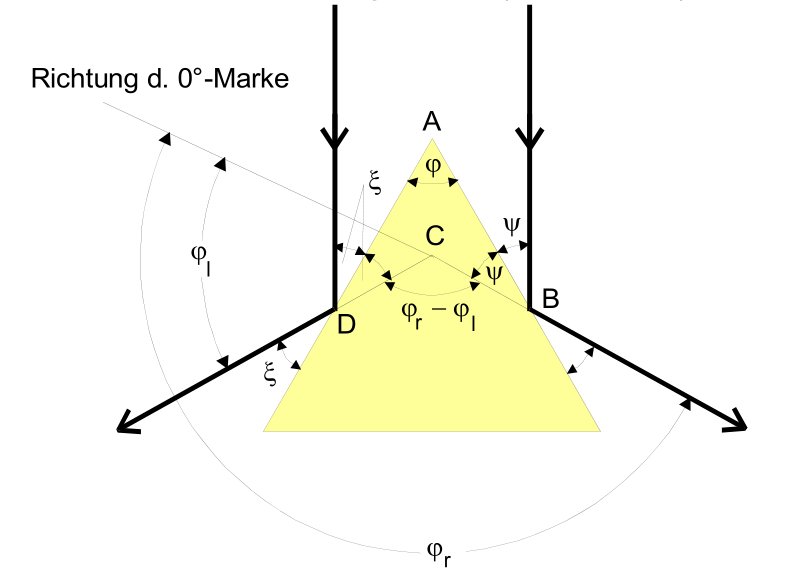
\includegraphics[height=4cm]{ressources/aufbau2.png}
  \caption{Abbildung zur Untersuchung des Winkels des Prismas. \cite{skript}}
  \label{fig:2}
\end{figure}

Dabei wird die Winkeldifferenz der beiden reflektierten Strahlen zueinander notiert und später über geometrische Überlegungen so verrechnet, dass der Winkel der Prismaecke bekannt sein wird.

\subsection{Bestimmung des Brechwinkels der Spektrallinien}

Um den Ablenkungswinkel der Spektrallinien zu messen, wird das Prisma zunächst so positioniert, dass die Kante des Strahlenbündels, wie in Abbildung \ref{fig:3}, an einer Seite des Prismas reflektiert wird, während der Rest das Prisma passiert.

\begin{figure}[H]
  \centering
  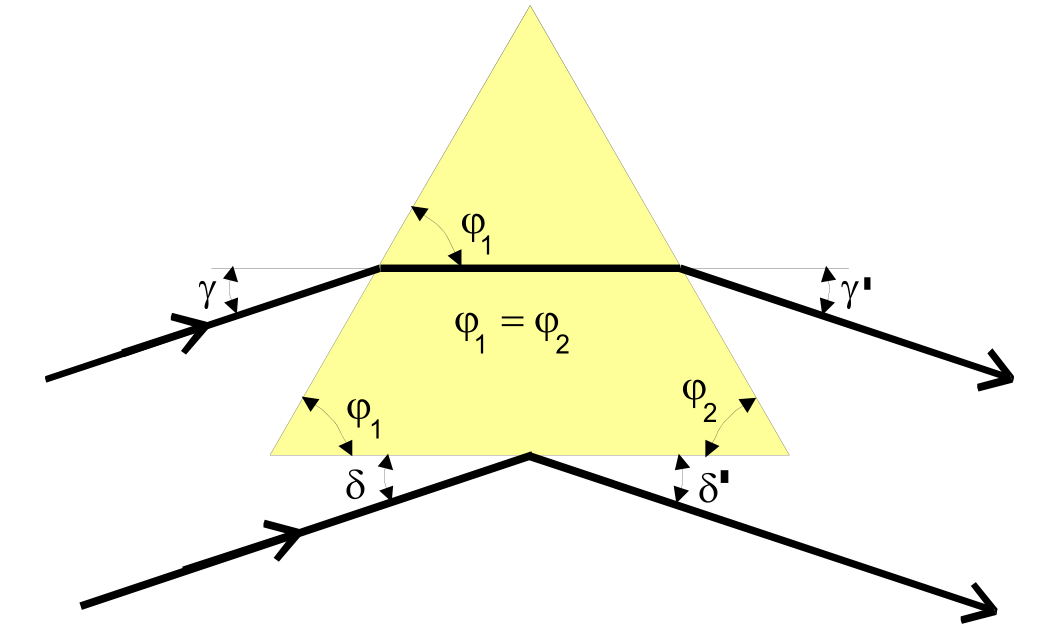
\includegraphics[height=4cm]{ressources/aufbau3.png}
  \caption{Abbildung zur Untersuchung des Winkels des Prismas. \cite{skript}}
  \label{fig:3}
\end{figure}

Nun sind das Beugungsbild und das Maximum des reflektierten Anteils zusehen.
Das Reflexionsmaximum wird jetzt über Drehung des Prismas mit der gewünschten Spektrallinie in Deckung gebracht.
Dieser Punkt wird nun angepeilt und es wird der Winkel notiert unter dem dies geschieht.
Dies wird spiegelsymmetrisch für die andere am oberen Winkel des Prismas liegende Seite durchgeführt.
Werden die beiden Winkel über geometrische Überlegungen geschickt verrechnet, ist das Ergebnis die gesammte Winkeländerung, welche die Brechung am Prisma hervorruft.
Jener Vorgang wird für alle Spektrallinien der Lampe wiederholt.
